%Dokumentklasse
\documentclass[a4paper,12pt]{scrreprt}
\usepackage[left= 2.5cm,right = 2cm, bottom = 4 cm]{geometry}
%\usepackage[onehalfspacing]{setspace}
% ============= Packages =============

% Dokumentinformationen
\usepackage[
	pdftitle={Single tone fingerprint analyse and reconstruction for creating highly dynamic sound libraries},
	pdfsubject={},
	pdfauthor={Karsten Dehren},
	pdfkeywords={},	
	%Links nicht einrahmen
	hidelinks
]{hyperref}


% Standard Packages
\usepackage[utf8]{inputenc}
\usepackage[english]{babel}
\usepackage[T1]{fontenc}
\usepackage{graphicx, subfig}
\graphicspath{{img/}}
\usepackage{fancyhdr}
\usepackage{lmodern}
\usepackage{color}
\usepackage[table]{xcolor}
\usepackage{multirow}
\usepackage{xcolor,colortbl}
\usepackage{amsmath}

\newcommand{\R}{\mathbb{R}}
\newcommand{\N}{\mathbb{N}}
\newcommand{\Nn}{\mathbb{N}_0}
\newcommand{\Z}{\mathbb{Z}}
\newcolumntype{d}{>{\columncolor{lightgray}}c}


% zusätzliche Schriftzeichen der American Mathematical Society
\usepackage{amsfonts}
\usepackage{amsmath}

%nicht einrücken nach Absatz
%\setlength{\parindent}{0pt}


% ============= Kopf- und Fußzeile =============
\pagestyle{fancy}
%
\lhead{}
\chead{}
\rhead{\slshape \leftmark}
%%
\lfoot{}
\cfoot{\thepage}
\rfoot{}
%%
\renewcommand{\headrulewidth}{0.4pt}
\renewcommand{\footrulewidth}{0pt}

% ============= Package Einstellungen & Sonstiges ============= 
%Besondere Trennungen
\hyphenation{De-zi-mal-tren-nung}


% ============= Dokumentbeginn =============

\begin{document}
%Seiten ohne Kopf- und Fußzeile sowie Seitenzahl
\pagestyle{empty}

\begin{center}
\begin{tabular}{p{\textwidth}}

\begin{center}
	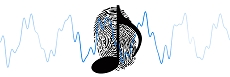
\includegraphics[scale=0.15]{img/note.png}
\end{center}
\\\\
\\\\
\hline
\begin{center}
\LARGE{\textsc{
Single note fingerprint analyse \\
and reconstruction for creating \\
highly dynamic sound libraries
}}
\end{center}
\\
\hline
\\



\begin{center}
\textbf{\Large{Paper}}
\end{center}


\begin{center}
for defining a new way of creating dynamic\\
and customizable sound library
\end{center}

\\
\\

\begin{center}
\large{\textbf{Karsten Dehren}}
\end{center}

\begin{center}
\large{April 2017}
\end{center}

\\

\\

\end{tabular}
\end{center}

% pagestyle für gesamtes Dokument aktivieren
\pagestyle{fancy}

\tableofcontents

\chapter{Motivation}
	During the development of a note editing software we had to decide between using a standard sound library based on wave (.wav) files or developing an own format. 
	\\The benefits of using a sound library based on standard wave files are first of all the easy set up of these files and then that for basic notes no additional calculations are necessary. But the disadvantages are that these libraries are usually inflexible and hard to edit at runtime and apart from that it takes a relative long time to load the files.
	\\In order to avoid these problems this paper will define a new strategy to manage and create sound libraries including a file format to define a fingerprints of each instrument and an optimized non-redundant data structure.
	
	\section{State of the art}
	The probably most common way of creating a sound library is a list of native wave files which contain the -- in average 3 to 5 second long -- data of one note. After being loaded the data can combined with existing informations by adding to overlay notes and concatenation to create a sounds or an entire song.
	\\This strategy works perfectly fine as long as there are no sound modulations necessary. But if the user wants to change the note -- for example a bended note on a guitar or a vibrating tone -- the software has to recalculate the file or to dynamically drop data segments to adjust the frequency. Neither of these strategies can maintain the sound quality because of a quick recalculation of sound files can’t start a detailed analyse what leads to a sound calculation with flawed or maybe even wrong parameters. And beside of that dropping data segments will directly influence the sound quality by ignoring details that could have had influenced the sound.
			
	\section{Benefits}
	The Dynamically Transformable Single Note Fingerprint file system and the Cloud Repository data structure offers developers an interface to build a flexible and composite sound library which enables users and developers to add own sounds to the application by recording only one note. The fingerprint -- extracted from the recorded note -- can be transferred into every note and in addition to that tone and note modulations cause just a minor increase of the calculation effort. Apart from that developers are able to create and add plug-ins to customize the functionalities and overall behaviour of the underlying system.
	

\chapter{Definitions}
	\section{Basic Definitions}
	\subsection{Sampling Rate}
	The Sampling rate $ SR $ defines the number of data units played every second. It will have the default value -- like a wave file sampling rate -- of $ 44100 $ data units per second.

	\subsection{Concert pitch}
	The concert pitch is a reference frequency to tune a group of instruments. From now on it will be called base frequency $ f_0 $ with the default value of
	\begin{equation*}
		f_0=440Hz
	\end{equation*} 
	\newpage
	\section{Musical definitions}
	\subsection{Amplitude}
	The Amplitude $ \mathcal{A} $ is a factor which defines the starting volume of a sine wave. It can only take values between 0 and 1.
	\begin{equation}\label{AmplitudeRef}
		\mathcal{A}\subset\R, \quad \mathcal{A}=[0, 1]
	\end{equation}

\subsection{Decay function}
	The decay $ \gamma $ is a linear or exponential function which defines how fast a sine wave will decay over time. With $ x,m,b\in\R $
	\begin{eqnarray}\label{DecayRef}
		\gamma(x)&=&m*(-x)+b\nonumber\\
		\gamma(x)&=&e^{f(x)}
	\end{eqnarray}
	
\subsection{Harmonic Series}
	A harmonic series is a list of frequencies which are contained in a note. Each frequency is a multiple of the base reference but they don't have to be a standard tone step.$ \Nn $
	\begin{eqnarray}
		&\exists n\in\N, F_B=F(n)&\\
		&F_{B_i}:=F_B*i, \quad \forall i\in\N&\\
		&&\\
		&\exists m\in\N, m>n, F_{B_i}=F(m) \Leftrightarrow 12|m-n&
	\end{eqnarray}
	\begin{eqnarray}
		F_{B_i}
		&=&F_B*i\\
		&=&F(n)*i\\
		&=&(f_0*(\sqrt[12]{2})^n)*i\\
		&=&(f_0*(\sqrt[12]{2})^{m-q})*i \qquad q\in\N\\
		&=&(f_0*(\sqrt[12]{2})^m*(\sqrt[12]{2})^{-q})*i \qquad 12|q\\
		&=&(f_0*(\sqrt[12]{2})^m*2^{p})*i \qquad p\in\N, p=\frac{q}{p}\\
	\end{eqnarray}
	\begin{center}
		\begin{tabular}{|ccccccccc|}
			\cline{1-2}
			First octave & $ C_0 $ & \multicolumn{0}{|}{}\\
			\cline{1-3}
			Second octave & $ C_1 $ & $ G_1 $ & \multicolumn{0}{|}{}\\
			\cline{1-5}
			Third octave & $ C_2$ & $E_2$ & $G_2$ & $\approx Bb_2 $&\multicolumn{0}{|}{}\\
			\hline
			Forth octave & $ C_3 $&$ D_3 $&$ E_3 $&$ \approx F_3 $&$ G_3 $&$ \approx Ab_3 $&$ \approx Bb_3 $&$ B_3 $\\
			\hline\hline
			\multicolumn{9}{|c|}{Example for base $ C_0 $}\\
			\hline
		\end{tabular}
	\end{center}

\subsection{Frequency calculation}
	$ n\in\Z $\\
	$ f_0=440 $Hz
	Octave:
	\begin{equation*}
		f_n=f_0*2^n
	\end{equation*}
		$ m\in\Z $
		12 half tone steps per octave
	\begin{equation}
		f_m=f_0*(\sqrt[12]{2})^m
	\end{equation}
	\begin{center}
		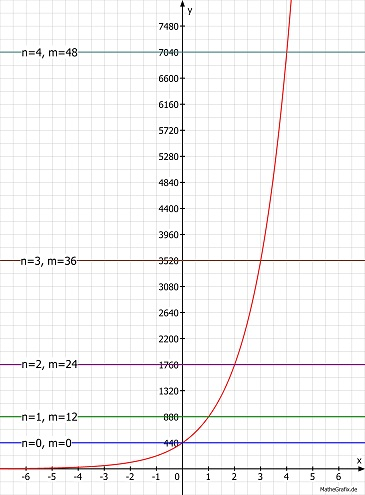
\includegraphics[scale=0.1]{img/frequencyFunction.jpg}
	\end{center}
	
	\subsection{Tone}
	A tone is a single sine wave with or without decay function. In addition to that it has an undefined factor or function which defines the wave amplitude. 
	\begin{equation}\label{ToneRef}
		T(x)=\mathcal{A} * \gamma(x) * sin(x) \quad x\in\R
	\end{equation}
	It can be combined with other tones by adding to overlap two tones.
	\begin{eqnarray}\label{ToneOperationRef}
		f:T \times T \rightarrow T, \quad A,B \mapsto A+B, \quad A,B\in T\nonumber \\
		A,B \in T \qquad f(A,B)=\sum_{i=0}^{\max\{|A| ,|B|\}} A(i)+B(i) 
	\end{eqnarray}

\subsection{Modulated Tone}
	A modulated tone is a specialization of standard tones. In addition to the tone properties it can have a frequency which is changing by time. The factor which changes the frequency will be defined in at least one additional function. IF the factor is defined by multiple functions they have to have a starting and terminating index to avoid function overlapping ambiguous information.
	\begin{equation}\label{ModToneRef}
		T(x)=\mathcal{A} * \gamma(x) * sin(f(x)), \quad x\in\R
	\end{equation}
	
	\subsection{Note}
	A note $ \phi $	is a vector of standard and modulated tones which will be played at the same time. These tones can be read individually or as unit what will transform them into a complex note. Beside of that the note defines the starting amplitudes of each tone.
	\begin{equation}\label{NoteRef}
		\phi=
		\begin{pmatrix}
			T_1\\
			T_2\\
			\vdots\\
			T_n
		\end{pmatrix}
	\end{equation}
	
\subsection{Complex note}
	A complex tone $ \widehat{\phi} $ is the sum of tones from one note.
	\begin{equation}\label{CompNoteRef}
	\widehat{\phi}=\sum_{i=1}^{n}T_i, \quad T_1, T_2, \dots, T_n\in\phi
	\end{equation}
	
\subsection{Sound}
	A Sound $ \Phi $ is matrix of Notes which defines their concatenation. 
	\begin{equation}\label{SoundRef}
		\Phi_{m,n}= 
		\begin{pmatrix}
			\phi_{11}&&\phi_{1n}\\
			&\ddots&\\
			\phi_{m1}&&\phi_{mn}

		\end{pmatrix}
	\end{equation}
	It can also be defined as vector of complex notes. In this case it will be called $ \widehat{\Phi} $.
	\begin{equation}\label{CompSoundRef}
		\widehat{\Phi}_n=
		\begin{pmatrix}
			\widehat{\phi}_1&\dots&\widehat{\phi}_n
		\end{pmatrix}
	\end{equation}
	\newpage
	\section{Sound fingerprint}
Sound fingerprints are the base for .DTSTF files. It contains the result of a wave analyse which will be defined later on. As a result of that it contains neither the analytical calculations nor a reconstruction definition.

\subsection{Contained information}
A sound fingerprint contains several informations. First of all the number of required sine waves what defines how many sine waves will be needed to create an appropriate note. In second place the wave definitions including a frequency and amplitude factor for each sine wave. And last of all the decay functions which will be defined by a function type and a decay factor.

\subsection{Data composition}
\textbf{\emph{Number of sine waves:}}
\begin{quote}
	This value will be defined by three numbers which declare how many sine waves -- with priority high, medium and low -- are required to create an appropriate note.
\end{quote}
\textbf{\emph{Frequency factor:}}
\begin{quote}
	The frequency factor $ f $ defines a value to modify a predefined base frequency $ \mathcal{F} $.
\end{quote}
\begin{eqnarray}
	& sin(f*\mathcal{F}) \quad f\in\N, \; \mathcal{F}\in\R_{>0}\nonumber \\
	(\ref{ToneRef})\Rightarrow & \; T(x)=\mathcal{A} * \gamma(x) * sin(f*\mathcal{F}) \quad x\in\R\nonumber
\end{eqnarray}
\textbf{\emph{Amplitude and decay function}}
\begin{quote}
	These values correspond to the definitions (\ref{AmplitudeRef}) and (\ref{DecayRef}).
\end{quote}

\subsection{File outlining}
\begin{equation}\label{DTSTFDataRef}
	\begin{tabular}{|c|c||d|}
		\hline 
		Section & Priority & Data\\
		\hline\hline
		\multirow{3}{*}{Number of required sine waves} & High & 4\\
		& Medium & 3\\
		& Low & 6\\
		\hline\hline
		Section & Frequency & Amplitude\\
		\hline\hline
		\multirow{13}{*}{Frequency and amplitude factor} 
		& 2 & 0,8\\
		& 4 & 0,6\\
		& 5 & 0,7\\
		& 8 & 0,6\\
		\cline{2-3}
		& 1 & 0,55\\
		& 3 & 0,5\\
		& 9 & 0,4\\
		\cline{2-3}
		& 6 & 0,3\\
		& 7 & 0,4\\
		& 10 & 0,35\\
		& 11 & 0,2\\
		& 12 & 0,12\\
		& 13 & 0,24\\
		\hline\hline
		Section & Type & Value\\
		\hline\hline
		\multirow{13}{*}{Decay function type and value}&
		\multirow{13}{*}{Exponential}
		& 1.3\\
		&& 1.5\\
		&& 1.8\\
		&& 1.1\\
		\cline{3-3}
		&& 1.9\\
		&& 1.6\\
		&& 2.2\\
		\cline{3-3}
		&& 1.9\\
		&& 1.0\\
		&& 2.1\\
		&& 2.6\\
		&& 1.4\\
		&& 1.7\\
		\hline
	\end{tabular}
\end{equation}
\begin{center}
	The data column shows information from the DTSTF format. The other two columns are for description.
\end{center}
	\newpage
	\section{File format .DTSTF}
	\subsection{File allocation}
	\subsection{File Header}
	\subsection{File Body}
	\subsection{Extended file outlining}
	\newpage
	

\end{document}